\documentclass{../industrial-development}
\graphicspath{{5-organization-of-developer-work/}}

\title{Методы и техники организации работы разработчика}
\author{Заплатин Егор Сергеевич, ПИ-21 МО}
\date{}

\begin{document}

\begin{frame}
  \titlepage
\end{frame}

\section{Введение}

\begin{frame} \frametitle{Рабочий процесс разработчика}
  \begin{itemize}
  \item Обдумывание задачи, поиск путей решения
  \item Изучение информации, чтение документации
  \item Написание кода
  \item Тестирование, поиск багов
  \item Участие во~встречах, планёрках и т.п.
  \item Чтение/написание писем, поиск/отметка задач в~трекере
  \item Общение с~коллегами
  \end{itemize}
\end{frame}

\begin{frame} \frametitle{Управление рабочим процессом}
Почему это важно:
  \begin{itemize}
  \item В течении дня возникает очень много задач
  \item Задачи постоянно меняются
  \end{itemize}
  \begin{block}{}
    Чтобы успевать всё сделать, разработчику приходится использовать методы управления задачами и методы управления временем
  \end{block}
\end{frame}

\section{Управление задачами}

\subsection{Разбиение задач на категории}

\begin{frame} \frametitle{Разбиение задач на категории}

  \begin{itemize}
  \item Когда задач становится много, сложно понять за~что взяться в~первую очередь
  \item Принцип, стоящий в~основе управления задачами --- составление списка задач
  \item Задачи нужно разбивать на~категории по~какому-то принципу, например, по~важности
  \end{itemize}
\end{frame}

\lecturenotes

Когда только начинаешь работать, то все ясно и понятно, задач не так много, есть представление как с ними работать. Но со временем приходит осознание, что задач накопилось очень много.

Принцип, который необходимо положить в основу — составление списка задач. Посмотрите на свои задачи и проставьте у каждой приоритет и сколько вы думаете затрать на нее времени. Если у вас слишком много задач, то подумайте, по какому критерию вы можете сократить рассматриваемый список задач. Например, вы можете отобрать только задачи в ближайшую версию исправления, только задачи в текущий спринт (если вы работаете по Scrum) и так далее. И именно с этим списком и стоит работать.

Итак, все дела списка разделите на 4 группы:
\begin{itemize}
\item Срочные и важные
\item Важные, но не срочные
\item Срочные, но неважные
\item Несрочные и неважные~\cite{TMHabr}
\end{itemize}

\begin{frame} \frametitle{Матрица Эйзенхауэра}
  \begin{table}
    \begin{tabular}{|c|p{0.4\linewidth}|p{0.4\linewidth}|}
		\hline
		 & Срочные дела & Несрочные дела \\
		\hline
		Важно & Разрешение кризисов & Планирование новых проектов \\
		 & Неотложные задачи & Оценка полученных результатов \\
		 & Проекты, у~которых подходят сроки сдачи & Определение новых перспектив \\
		\hline
		Неважно & Прерывания, перерывы & Рутинная работа \\
		 & Некот. телеф. звонки & Некоторые письма \\
		 & Некоторые совещания & Некот. телеф. звонки \\
		 & Обществ. деятельность & Развлечения \\
		\hline
    \end{tabular}
  \end{table}
\end{frame}

\begin{frame} \frametitle{Правила работы с задачами}
  \begin{itemize}
  \item Для каждой задачи ставится лимит времени на~её решение
  \item Шаг планирования ровно один рабочий день
  \item Время отдыха также планируется
  \item Просчитываются риски и закладывается на~них время
  \item Составляется список минимум и список максимум
  \item Список нужно где-то зафиксировать
  \end{itemize}
\end{frame}

\lecturenotes

Теперь у каждой задачи проставим время, которое мы потратим на ее решение. И, помня, что у нас всего 8 рабочих часов в день, составим список задач на сегодня. Список стоит составлять накануне вечером либо, как только вы придете на работу.

Очень важно, что все задачи вы должны планировать исходя из того, чтобы сделать их ровно в рабочий день. Никак не больше. Не планируйте работать сверхурочно без крайней необходимости. Это приведет только к усталости. Лучше потратить свободное время на саморазвитие и чтение профессиональной литературы.

Не забудьте учесть, что у вас чистых рабочих меньше, чем 8 часов. Нужно учесть время на перерывы, отдых физический. Разработчик не должен все время сидеть за компьютером. Запланируйте, что, хотя бы по 15 минут каждые два часа вы будете выгонять себя, вставать и просто пройдитесь и проветритесь. При этом эффективность работы только вырастет. Это поможет, не теряя темпа, успеть сделать то, что не смог бы сделать без отдыха.
НО, не нужно злоупотреблять. На перерыв можно потратить максимум полчаса, иначе мозг слишком расслабляется и теряется рабочий настрой.

В этом списке должны быть не только важные и долгие задачи, но и лёгкие, быстрые, чтобы на них можно было переключить внимание, расслабиться. Для разработчика это крайне важно. Задачи можно выполнять в любом порядке, но тем не менее рекомендуется начинать с важных. И обязательно начать с тех, которые меньше всего хочется делать.

Установите лимит времени на решение задачи. Если вы безрезультатно (именно безрезультатно!) сидите над задачей больше 2 часов, то пришла пора переключиться на другую задачу. У вас в списке есть такие задачи в разряде простых. Мы их специально для этого и включили.

Составьте список минимум и список максимум. Список минимум должен быть выполнен обязательно. К тому же при его выполнении вы почувствуете удовлетворенность собой. Список максимум нужен, если останется время. Если вы не успели свою программу минимум, то вы неправильно оцениваете свои силы, нужно подходить к этому более тщательно.
Если вы научились выполнять список минимум и у вас уже который день подряд остается время на список максимум, то пора увеличивать список минимум. И да, опять же — снова смотреть почему вы неправильно оценили время на задачи.

Зафиксируйте где-то список: на бумаге или в электронной версии. Но так, чтобы он был у вас перед глазами. Это поможет видеть сколько уже сделано и сколько еще осталось. Также вы получите эмоциональное удовлетворение при вычеркивании очередной задачи из списка, а это даст дополнительную мотивацию. Поэтому очень важно именно вычеркивать задачи, а не удалять.

Запланируйте время на форс-мажоры. Как гласит закон Мёрфи «если что-то может случиться, то это обязательно случится». Как правило, разработчики чувствуют такие моменты~\cite{TMHabr}.

\subsection{Разбиение задач на подзадачи}

\begin{frame} \frametitle{Разбиение задач на подзадачи}
  \begin{itemize}
  \item Множество задач, нужно раздробить на~понятные целые единицы работы
  \item Разбиение на~подзадачи позволяет отслеживать прогресс
  \item Каждая небольшая решённая задача — это~успех, который мотивирует
  \item Инструменты визуализации и~планирования вроде досок и~заметок помогают видеть действительно выполненную работу и~потраченное на неё время
  \end{itemize}
\end{frame}

\lecturenotes

Когда мы подходим к чему-то со всей серьёзностью, когда мы работаем с большим количеством людей, мы должны тщательно спланировать каждый свой шаг. Это поможет избежать ошибок, видеть свой прогресс и отслеживать реализацию.

Это касается и основных трудовых задач. К примеру, нужно разбить приложение на модули, отделить графический интерфейс от бэкенда. И работать над каждым модулем отдельно.
Каждый модуль разбивается на конкретные задачи.

И даже это множество задач, нужно раздробить на понятные целые единицы работы. Зачем? Чтобы не получилось нечто ужасное.

Эту задачу изначально нужно было разбить на подзадачи, чтобы видеть прогресс. Я имею ввиду, что каждая небольшая решённая задача — это успех, который мотивирует. А огромная задача, прогресс которой невозможно отследить в течение 2-х дней — это подавляющая стремления проблема.

Я проделал огромную работу, но результат своих трудов увидел только в конце задачи. Это очень утомляет, когда не видишь успех, когда не можешь выделить конкретные решённые вопросы.

Всегда разбивайте задачи на подзадачи. Смотрите за своим прогрессом и мотивируйте себя им. Используйте различные инструменты планирования, вроде досок и заметок. Это поможет вам видеть свою действительно выполненную работу и потраченное время. А в дальнейшем это поможет вам “на лету” оценивать задачи~\cite{TasksMedium}.

\begin{frame} \frametitle{Как сделать, чтобы разбиение на подзадачи работало}
  \begin{itemize}
  \item Не~стоит ставить совсем простые задачи, их~решение даёт мало мотивации
  \item Важно не~отвлекаться от~выполнения модели предсказания
  \item Задачи не~должны превышать 3 суток, а~лучше всего максимум несколько часов, и~обязательно должны подтверждаться фактом их~достижения
  \end{itemize}
\end{frame}

\lecturenotes

Основной механизм функционирования человека в нашей сложной системе поведения, это умение предсказывать (модели предсказания, созданные нашим опытом). 

Возможность предсказывать лежит в основе создания коротких целей. Однако не всё так просто.
Если мы создаем предсказание с максимальной вероятностью (100\%), то оно не создает позитивной мотивации.
Мотивация же относится к тем случаям, когда предсказание не гарантирует достижение цели, но мы своими усилиями, на основе предсказания, всё же достигаем позитивного результата. Притом сила мотивации пропорциональна соотношению двух факторов: «бонус» и вероятность.
Точно также действуют и короткие задачи.

Когда вы ставите короткую задачу, она не должна быть 100\% предсказанной, то есть вы не должны детально четко знать каждый шаг по ее достижению. Это снижает «бонус», которым нас мотивирует подсознание. Если вы будете это знать, то такое задание не вызывает позитива, но является растратой ресурсов, так создается «рутина».

Если вы ставите короткую задачу средней предсказанности и реализуете ее точно со своей моделью предсказания, вы получаете свой позитив.

Собственно почему тогда задачи нужны именно короткие?

Дело в том, что поставив цель, вы создаете предсказание ее достижения, и подсознание по умолчанию считает, что в реализацию предсказания входят все действия между ее постановкой и окончательным результатом.

Если вы предсказываете, что сделаете модуль за 30 минут, подсознание дает мотивацию на достижение, так как считает, что вы будете непрерывно заниматься этим модулем и имеете вероятность его закончить именно через 30 минут.
Если же каждые 5 минут вас начинают «дергать», то подсознание может в результате понизить мотивацию, как эти «дерганья» начинают включаться в модель предсказания, и тем самым ваш модуль «стОит» для подсознания уже гораздо дороже, а такую цену оно возможно не готово платить.

Если такие случаи будут повторяться, то подсознание вырабатывает уже новое предсказание, которое не способно вас будет замотивировать даже на этот простой модуль.

Именно поэтому в таких случаях важно или не отвлекаться от выполнения модели предсказания, или уметь очень сильно и четко переключать своё сознание, чтобы также и переключалось предсказание. Это довольно сложно сделать, если вас переключают на другие дела, требующие умственных усилий, но гораздо легче, если эти переключения идут в область 100\% предсказаний, например, отлучиться в туалет.

Всё это гораздо сложнее реализовать для больших задач, следовательно, на большие задачи требуются более сложные методы мотивации и конечно разбиение их на подзадачи.

В идеале короткие мотивационные задачи не должны превышать 3 суток, а лучше всего максимум несколько часов, и обязательно должны подтверждаться фактом их достижения, чтобы подсознание фиксировало, что предсказание успешно завершено~\cite{TasksHabr}.

\begin{frame} \frametitle{Работа со сложными задачами}
  \begin{itemize}
  \item Сложная задача должна стоять первой в~списке
  \item Если появилось желание отложить задачу на~потом, это~знак, что~ей~нужно заняться прямо сейчас
  \item Можно представлять, что~осталась только одна эта~задача
  \item Если нужна концентрация стоит включить «турбо режим»
  \end{itemize}
\end{frame}

\lecturenotes

Рассмотрим работу с тяжелыми задачами. Теми, которые почему-то кажутся неподъемными. Они пугают либо тем, что непонятно как к такой задаче подступиться, либо тем, что не хочется общаться с ее автором/заказчиком. Следующие несколько правил именно о таких задачах.

Если у вас появилась неподъемная задача, за которую вы не хотите приниматься или не знаете как оценить, то она должна встать первой в вашем списке. Это потенциальная черная дыра и может оказаться неразрешимой для вас или слишком затратной по времени, что грозит тем, что вы ее просто не успеете сделать. Начните с нее, возвращайтесь к ней в течение дня, пока она не станет для вас понятной, попробуйте разбить ее на более мелкие. 
Также может помочь просто рассказать кому-то из коллег о задаче, отобразить ее на доске или даже просто рассказать вслух о проблеме.
Как только хочется отложить задачу на завтра, то это знак, чтобы заняться ей прямо сейчас.

Старайтесь выполнить задачи так, чтобы если у вас и осталась эта неподъемная задача, то только она одна. Иначе у вас не будет удовлетворения и будет зависание на одной этой задаче и ряд невыполненных других.

Если вам нужна концентрация, используйте турбо-режим. Он действительно работает. Для этого на определенное время отключите все средства связи (skype, icq и др.), поставьте табличку, чтобы вас не отвлекали, оденьте наушники и не реагируйте ни на что. В эти 25 минут вы занимаетесь только решением одной конкретной задачи. Не отвлекайтесь ни на что. Главное не злоупотреблять этим, особенно в крупных компаниях~\cite{TMHabr}.

\section{Управление рабочим временем}

\subsection{Принципы тайм-менеджмента для разработчика}

\begin{frame} \frametitle{Принципы тайм-менеджмента для разработчика}
  \begin{itemize}
  \item Отслеживать все~задачи, вести журнал задач
  \item Делегировать задачи, когда~это~возможно
  \item Не стремиться к~идеальному результату
  \item Планировать работать во~время, когда~количество отвлечений будет минимально
  \item Планировать время на~расслабление и~отдых
  \item Очень важно вознаграждать себя за~выполнение задач
  \end{itemize}
\end{frame}

\lecturenotes

Если вы ничего не планируете сейчас, не беспокойтесь, вы можете это сделать позже. Просто отследите, что вы делаете на бумаге, листе Excel или используете программное обеспечение для управления задачами. Обновляйте список каждые два часа или, по крайней мере, в конце дня в начале. Это поможет вам найти общие прерыватели и повторяющиеся задачи, таким образом, вы сможете планировать вещи на будущее. Даже одна неделя дневного отслеживания может рассказать о том, как мы живем.
Посмотрите на свой журнал времени и попытайтесь выяснить, что действительно не нужно делать, что может сделать кто-то другой, работу, которую можно сделать более эффективно или быстро, действия, которые тратят время других и т. Д.

Делегировать задачи, когда это возможно
Если кто-то, кто может принять участие в вашей работе, не стесняйтесь поделиться с ним некоторой работой. Опишите задачу четко.
В многопроектной среде работа всей команды не может быть распределена поровну каждому члену. Кому-то придется делать больше и кого-то меньше. Используя теорию ограничений Голдрата, проект не может быть завершен до тех пор, пока самый медленный член не завершит свою работу. Таким образом, делегацию следует продвигать внутри команды, причем не только от менеджера до разработчика. Этот процесс может быть эффективен только в командах с честным и открытым общением.

Идеально не лучше, чем хорошо.
Например, при написании кода важно закончить вовремя, чем беспокоиться о идеальном решении, которое подходит для всех. Завершите работу, дополнительные функции можно добавить позже.  Используйте модульные тесты, это может улучшить качество и ускорить разработку.

Определите свое время
Человек - это социальное существо, мы имеем дело с людьми каждый день и час. У нас есть коллеги, друзья или родственники. Они могут помогать или замедлять вас различными способами. Кто-то может спросить вас напрямую, по телефону, через мессенджер или по электронной почте. Это приводит к прерываниям, а также затратам времени. Прерывание в течение 6 -- 9 минут обычно требует дополнительных 4 -- 5 минут для восстановления. Пять прерываний будут стоит в час. Всегда хорошо думать о способах уменьшить частоту таких перерывов. Единственный способ сократить такие затраты времени - найти повторяющиеся отходы времени. Как только вы получите всю картину, легко решить, где сэкономить и где потратить.

Планирование расслабление и отдыха
Не ожидайте высокой производительности, если вы устали. Сон заряжает наши мозги и помогает нам мыслить более четко. Планируйте свой день адекватно, не забывайте спать.

Разработчики обычно сидят 8 часов в день или более на рабочем месте рядом с компьютером. Это приводит к эмоциональным и физическим заболеваниям. Один из наших уязвимых органов --- это глаза. Работа за монитором в течение длительного времени разрушает наше зрение. Чтобы уменьшить пагубное влияние на глаза, существует много методов тренировки глаз. Запланируйте его ежедневно, перед ужином или в любое другое удобное время.

Награди себя
Каждый ожидает награду или похвалу за свою работу, особенно за то, что он что-то закончил. Отсутствие награды может убить наше желание работать. Это обычно приводит к снижению производительности. Вот почему мы предпочитаем работать на других, чем делать что-то для себя. Обещайте себе награду после выполнения задания или завершения работы. Например, позвольте себе посмотреть интересный фильм, как только вы закончите разработку страницы или новой функции, или съешьте сладости или что-нибудь еще~\cite{TMCodeProject}.

\subsection{Персональные спринты}

\begin{frame} \frametitle{Персональные спринты}
  \begin{itemize}
  \item Можно применять технику «спринт» из Agile
  \item Устраивать несколько 45-минутных спринтов в~день
  \item Сообщить своей команде, чтобы вас~в~это время не~отвлекали
  \end{itemize}
\end{frame}

\lecturenotes

Многие команды разработчиков в наши дни слышали об Agile и, скорее всего, о том, что такое «спринт». Поэтому для большинства людей эта концепция должна быть хорошо известна. Как мы применим это к нашему личному времени работы?

Легко! Планируйте это. Начните в определенное время с определенной работы. И просто работайте над какой-то конкретной задачей. Это может быть несколько 45-минутных блоков. Но планируйте свой день для работы над конкретными задачами в определенное время, а затем выполняйте эту деятельность и минимизируйте прерывания в вашем спринте.

Сообщайте своей команде, что вы находитесь в процессе «персонального спринта», чтобы люди научились не прерывать вас, пока вы пытаетесь достичь состояния потока~\cite{TMSeimer}.

\subsection{Техника Pomodoro}

\begin{frame} \frametitle{Техника Pomodoro}
  \begin{itemize}
  \item Используется таймер для~запланированных действий
  \item Время одной Pomodoro подбирается индивидуально
  \item Мелкие задачи группируются
  \item Крупные задачи разбиваются на~мелкие
  \item Чем~больше применяется эта~техника, тем~точнее получается планировать время
  \item Игнорируются отвлечения в~процессе сеанса Pomodoro
  \end{itemize}
\end{frame}

\lecturenotes

Несколько правил техники «Pomodoro» в тайм менеджменте:
\begin{itemize}
\item Использовать таймер для запланированных действий
\item Просматривайте временные затраты, чтобы лучше оценивать в будущем
\item Игнорируйте попытки отвлечения внимания во время сеансов Pomodoro~\cite{TMSeimer}
\item Известно, что продуктивность у всех людей разная, так же как и способность к концентрации, поэтому временные рамки при выполнении техники могут немного сдвигаться в ту или другую сторону. Например, кто-то может легко работать, не отвлекаясь, в течение 45 минут, тогда его «помидор» будет равняться именно этому времени. А кому-то 5 минут отдыха совсем не хватает, чтобы «перезагрузиться, тогда он может для себя установить 10-15 минутные перерывы
\item Если у вас есть задачи, на выполнение которых потребуется всего несколько минут, сгруппируйте их вместе в один «помидор», чтобы за 25 минут можно было решить все эти мелкие вопросы
\item И, наоборот, если на выполнение какого-то задания вам не хватит пяти 25-минуток, тогда следует разделить его на более мелкие задачи
\item Сам «помидор» делить на части запрещается, и прерываться во время «съедания помидора» тоже нельзя. Если вы вынужденно прервались более чем на минуту, перезапустите свой таймер и начните отсчет времени сначала~\cite{Pomidoro}
\end{itemize}

\begin{frame} \frametitle{Этапы техники Pomodoro}
  \begin{itemize}
  \item Постановка конкретной задачи
  \item Подготовка подручных средств: блокнот, ручка и~таймер
  \item Установка таймера на~25--45 минут
  \item Непрерывная работа в~течение 25--45 минут
  \item Перерыв на~5 минут
  \item Ещё 3 помидора с~пятиминутными перерывами
  \item Перерыв на~15--30 минут
  \end{itemize}
\end{frame}

\lecturenotes

Основные этапы работы по «методу помидора»:
\begin{enumerate}
  \item Постановка конкретной задачи, которой вы планируйте заняться непременно сегодня. В идеале, вы должны постоянно ставить перед собой цели и определять примерное время, в течение которого они будут достигнуты. А чтобы этого добиться, нужно определять еще задачи,  выполнение которые приведет вас к желаемым целям.  Совокупность таких задач – это ваш план на день
  \item Подготовка подручных средств, к которым отнесем блокнот, ручку и таймер (или будильник). Это самое простое, что всегда находится под рукой. Для более «продвинутых» можно посоветовать воспользоваться компьютерными программами, разработанными специально для управления временем по технике «помидор»
  \item Установка таймера на 25 минут. Считается, что это оптимальное время, чтобы сконцентрироваться на конкретной проблеме и, удерживая внимание, продуктивно над ней поработать без потери концентрации
  \item Непрерывная работа в течение 25 минут. Пока не раздастся сигнал таймера, свидетельствующий об окончании деятельности, вы должны сделать все, чтобы не отвлекаться на телефонные звонки, Интернет, проверку своего электронного ящика и соцсетей
  \item Перерыв на 5 минут. Поставив галочку о завершении сессии, полностью отвлекитесь от работы, переключившись на другой вид деятельности, непременно расслабляющий
  \item Непрерывная работа в течение очередных 25 минут. Каждая такая 25-минутная работа называется помидором. Проделанная работа в течение этого времени = 1 помидор, который вы «съели»
  \item Второй перерыв на 5 минут
  \item Третий «помидор» на 25 минут
  \item Третий перерыв на 5 минут
  \item Четвертый «помидор» на 25 минут
  \item Перерыв на 15-30 минут. После такой трудоемкой деятельности непременно нужно сделать более продолжительный перерыв. 15-30 минут – это оптимальное время для отдыха. После него можно с новыми силами взяться за выполнение новых заданий~\cite{Pomidoro}
\end{enumerate}

\subsection{Getting Things Done method}

\begin{frame} \frametitle{Getting Things Done method}
  \begin{block}{Определение}
    Getting Things Done, GTD (в~переводе с~англ. — «доведение дел до завершения») --- методика повышения личной эффективности, созданная Дэвидом Алленом
  \end{block}
  \begin{itemize}
  \item GTD основана на~принципе, гласящем, что~человек должен освободить свой~разум от~запоминания текущих задач, перенеся сами~задачи и~напоминания о~них на~внешний носитель
  \end{itemize}
\end{frame}

\begin{frame} \frametitle{Фильтры на список дел}
В первую очередь нужно выбрать основное среди всех задач:
  \begin{itemize}
  \item Выбрать начатые, но~не~завершённые задачи
  \item Выбрать дела, вызывающие наибольшее беспокойство
  \item Выбрать дела, которые не~хочется выполнять, и,~которые всё~время откладываются
  \item Выбрать рутинные дела, в~том числе бытовые
  \end{itemize}
\end{frame}

\lecturenotes

Прежде всего, нужно установить ограничения, выбрав основное среди всех задач. Оставляя главное, вы высвобождаете время и силы и создаёте импульс для действий с гораздо меньшими трудозатратами, чем, когда вы держите в голове все мелочи. Есть рутина, есть важные проекты, есть планы на будущее. При этом во всех перечисленных категориях есть главное. Чтобы его выделить, нужно выполнить несколько шагов:
  \begin{itemize}
  \item Выбрать начатые, но не завершённые задачи
  \item Выбрать дела, вызывающие наибольшее беспокойство
  \item Выбрать дела, которые не хочется выполнять и которые всё время откладываются
  \item Выбрать рутинные дела, в том числе бытовые
  \end{itemize}
Как правило, основное находится первых трёх группах. Соответственно, первоочередное внимание следует уделить беспокоящим и незавершённым делам — ведь не даром точный перевод Getting Things Done — «довести дела до завершения»~\cite{GTDHabr}.

\begin{frame} \frametitle{Упорядочивание каналов коммуникации}
  \begin{itemize}
  \item Установить всплывающие оповещения для~писем на~e-mail, на~которые можно посмотреть краем глаза
  \item Разделить все~коммуникации по~контексту: Skype, мобильные звонки, городской телефон, общение через~почту и~т.д. Отвести определённое время на~коммуникацию внутри каждого канала
  \item Какие-то интересные темы и~обсуждения в~интернете, не~имеющие никакого отношения к~текущей задаче, откладываются в~закладки
  \item Интересы распределяются по~мере их~значимости по~отношению к~текущим проектам, краткосрочным и~долгосрочным целям
  \end{itemize}
\end{frame}

\lecturenotes

Неважно, фрилансер или программист, работает удалённо или в команде, он постоянно находится в поле коммуникации: звонки заказчиков, вопросы руководства, запросы пользователей и коллег, информационные сообщения от поставщиков SDK и проч… Эти коммуникации нельзя назвать малозначительными, но их нужно уметь грамотно обрабатывать.
  \begin{itemize}
  \item Перестаньте проверять e-mail каждые 5 минут — установите всплывающие оповещения, на которые можно глянуть краем глаза. Разместите почту по папкам и прочитывайте по мере актуализации в конкретный момент.
  \item Разделите все коммуникации по контексту: Skype, мобильные звонки, городской телефон, общение через почту и т.д… Отведите определённое время на коммуникацию внутри каждого канала
  \item Проверьте рабочие и личные чаты. Возможно, если вам без конца пишет ваш новый сотрудник или задаёт одни и те же рабочие вопросы старый коллега, стоит попросить их подготовить вопросы, выделить время на общение и разъяснить все сложные моменты
  \item Понаблюдайте за своим веб-браузером. Разработчики часто смотрят профильные темы на форумах или специализированных сайтах. Там их подстерегают интересные темы и обсуждения, не имеющие никакого отношения к текущей задаче. Лучше отложить чтение действительно интересной темы, воспользовавшись закладками в браузере или специальными утилитами для хранения ссылок (например, дополнение Pocket, которое можно также установить как приложение на мобильном устройстве и синхронизировать закладки)
  \item Заведите записную книжку и/или приложение, где вы будете записывать все задачи с метками срочности и важности. GTD для управления делами вводит понятия времени, контекста (места), действия. Чтобы правильно расставить приоритеты задач, представьте себе простой фильтр, как в Excel, например. Присвойте каждой задаче параметр времени (по часам или времени суток), места (дом, работа, улица, спортзал, магазин и т.д.). А затем разделите задачи примерно таким образом: «запросить комментарии к ТЗ — работа — 14:00» или «позвонить в шиномонтаж — улица — вечер». Для подобных записей существует много приложений: от планировщика заданий в Windows, который можно использовать для своих целей до Evernote, Rainlendar и тщательно прописанных напоминаний на смартфон
  \end{itemize}
Уверенность в том, что у вас есть такой список, гарантированно снизит уровень тревожности и поможет сосредоточиться на решении каждой из задач.

Есть и более глобальная проблема, которая также затрагивает разработчиков любого типа занятости. Сегодня почти каждую неделю выходят новые инструменты, гайды, утилиты для разработчиков, то и дело появляются сообщения о новых версиях фреймворков, новых библиотеках и даже новых языках программирования. Вся эта информация вызывает чрезвычайный интерес профессионалов, а иногда даже увлекает и заставляет попробовать что-то новое (создать простое мобильное приложение, написать «Hello, world!» на Brainfuck или собрать новый опенсорсный проект). Выход один: распределять интересы по мере их значимости по отношению к текущим проектам, краткосрочным и долгосрочным целям. Фокусировка на одной задаче даёт возможность повысить личную продуктивность, освободить время и приступить к изучению новой информации~\cite{GTDHabr}.

\begin{frame} \frametitle{Управление рабочим процессом}
  \begin{itemize}
  \item Сбор
  \item Обработка
  \item Организация
  \item Обзор
  \item Действия
  \end{itemize}
\end{frame}

\lecturenotes

Первая главная модель — управление рабочим процессом, используется для того, чтобы взять под контроль все задачи и поручения. Управление рабочим процессом состоит из пяти фаз:
\begin{itemize}
\item Сбор
\item Обработка
\item Организация
\item Обзор
\item Действия~\cite{GTDWikipedia}
\end{itemize}

\begin{frame} \frametitle{Сбор информации}
  \begin{itemize}
  \item Фиксация всего более-менее важного на~бумаге или~другом носителе (корзине)
  \item Задачи делятся по~разделам, соответствующим каждому проекту, отделяются личные документы от~рабочих
  \item Все корзины освобождаются (обрабатываются) по~крайней мере раз~в~неделю
  \end{itemize}
\end{frame}

\lecturenotes

Сбор информации. Нужно собрать все задачи— просто взять и записать ручкой или в текстовый файл все свои рутинные, незавершённые, глобальные дела. При этом важно помнить, что, например, за задачей «Написать отчёт в Fast Report для ООО «Снеговик» скрывается несколько важных и требующих внимания подзадач: собрать требования с клиента, составить и утвердить ТЗ, запросить массив данных для тестирования отчёта и т.д… Необходимо записывать абсолютно все задачи — чуть позже вы их сгруппируете.
Обратите внимание не только на те проекты, которые есть в памяти, но и на те, которые находятся в компьютере — зачастую там не меньше хаоса, чем в мыслях. Стоит разделить файлы по папкам, соответствующим каждому проекту, отделить личные документы от рабочих~\cite{GTDHabr}. 

Продуктивность без стресса начинается с процесса разгрузки разума, которое заключается в фиксации всего более-менее важного на бумаге или другом носителе — в том, что Аллен называет корзиной: физический ящик для приёма сообщений, электронный почтовый ящик, диктофон, ноутбук, карманный компьютер, или их комбинация. Суть в том, чтобы выкинуть из головы всё более-менее важное на удобный носитель для последующей обработки. Все корзины должны быть освобождены (обработаны) по крайней мере раз в неделю. Аллен не настаивает на каком-то определённом методе сбора, но делает акцент на важности регулярного освобождения корзины. Любое место хранения (физический, электронный почтовый ящик, магнитофон, ноутбук, карманный компьютер, и т.д), приемлемо, если оно регулярно обрабатывается~\cite{GTDWikipedia}.

\begin{frame} \frametitle{Процесс обработки}
  \centerline{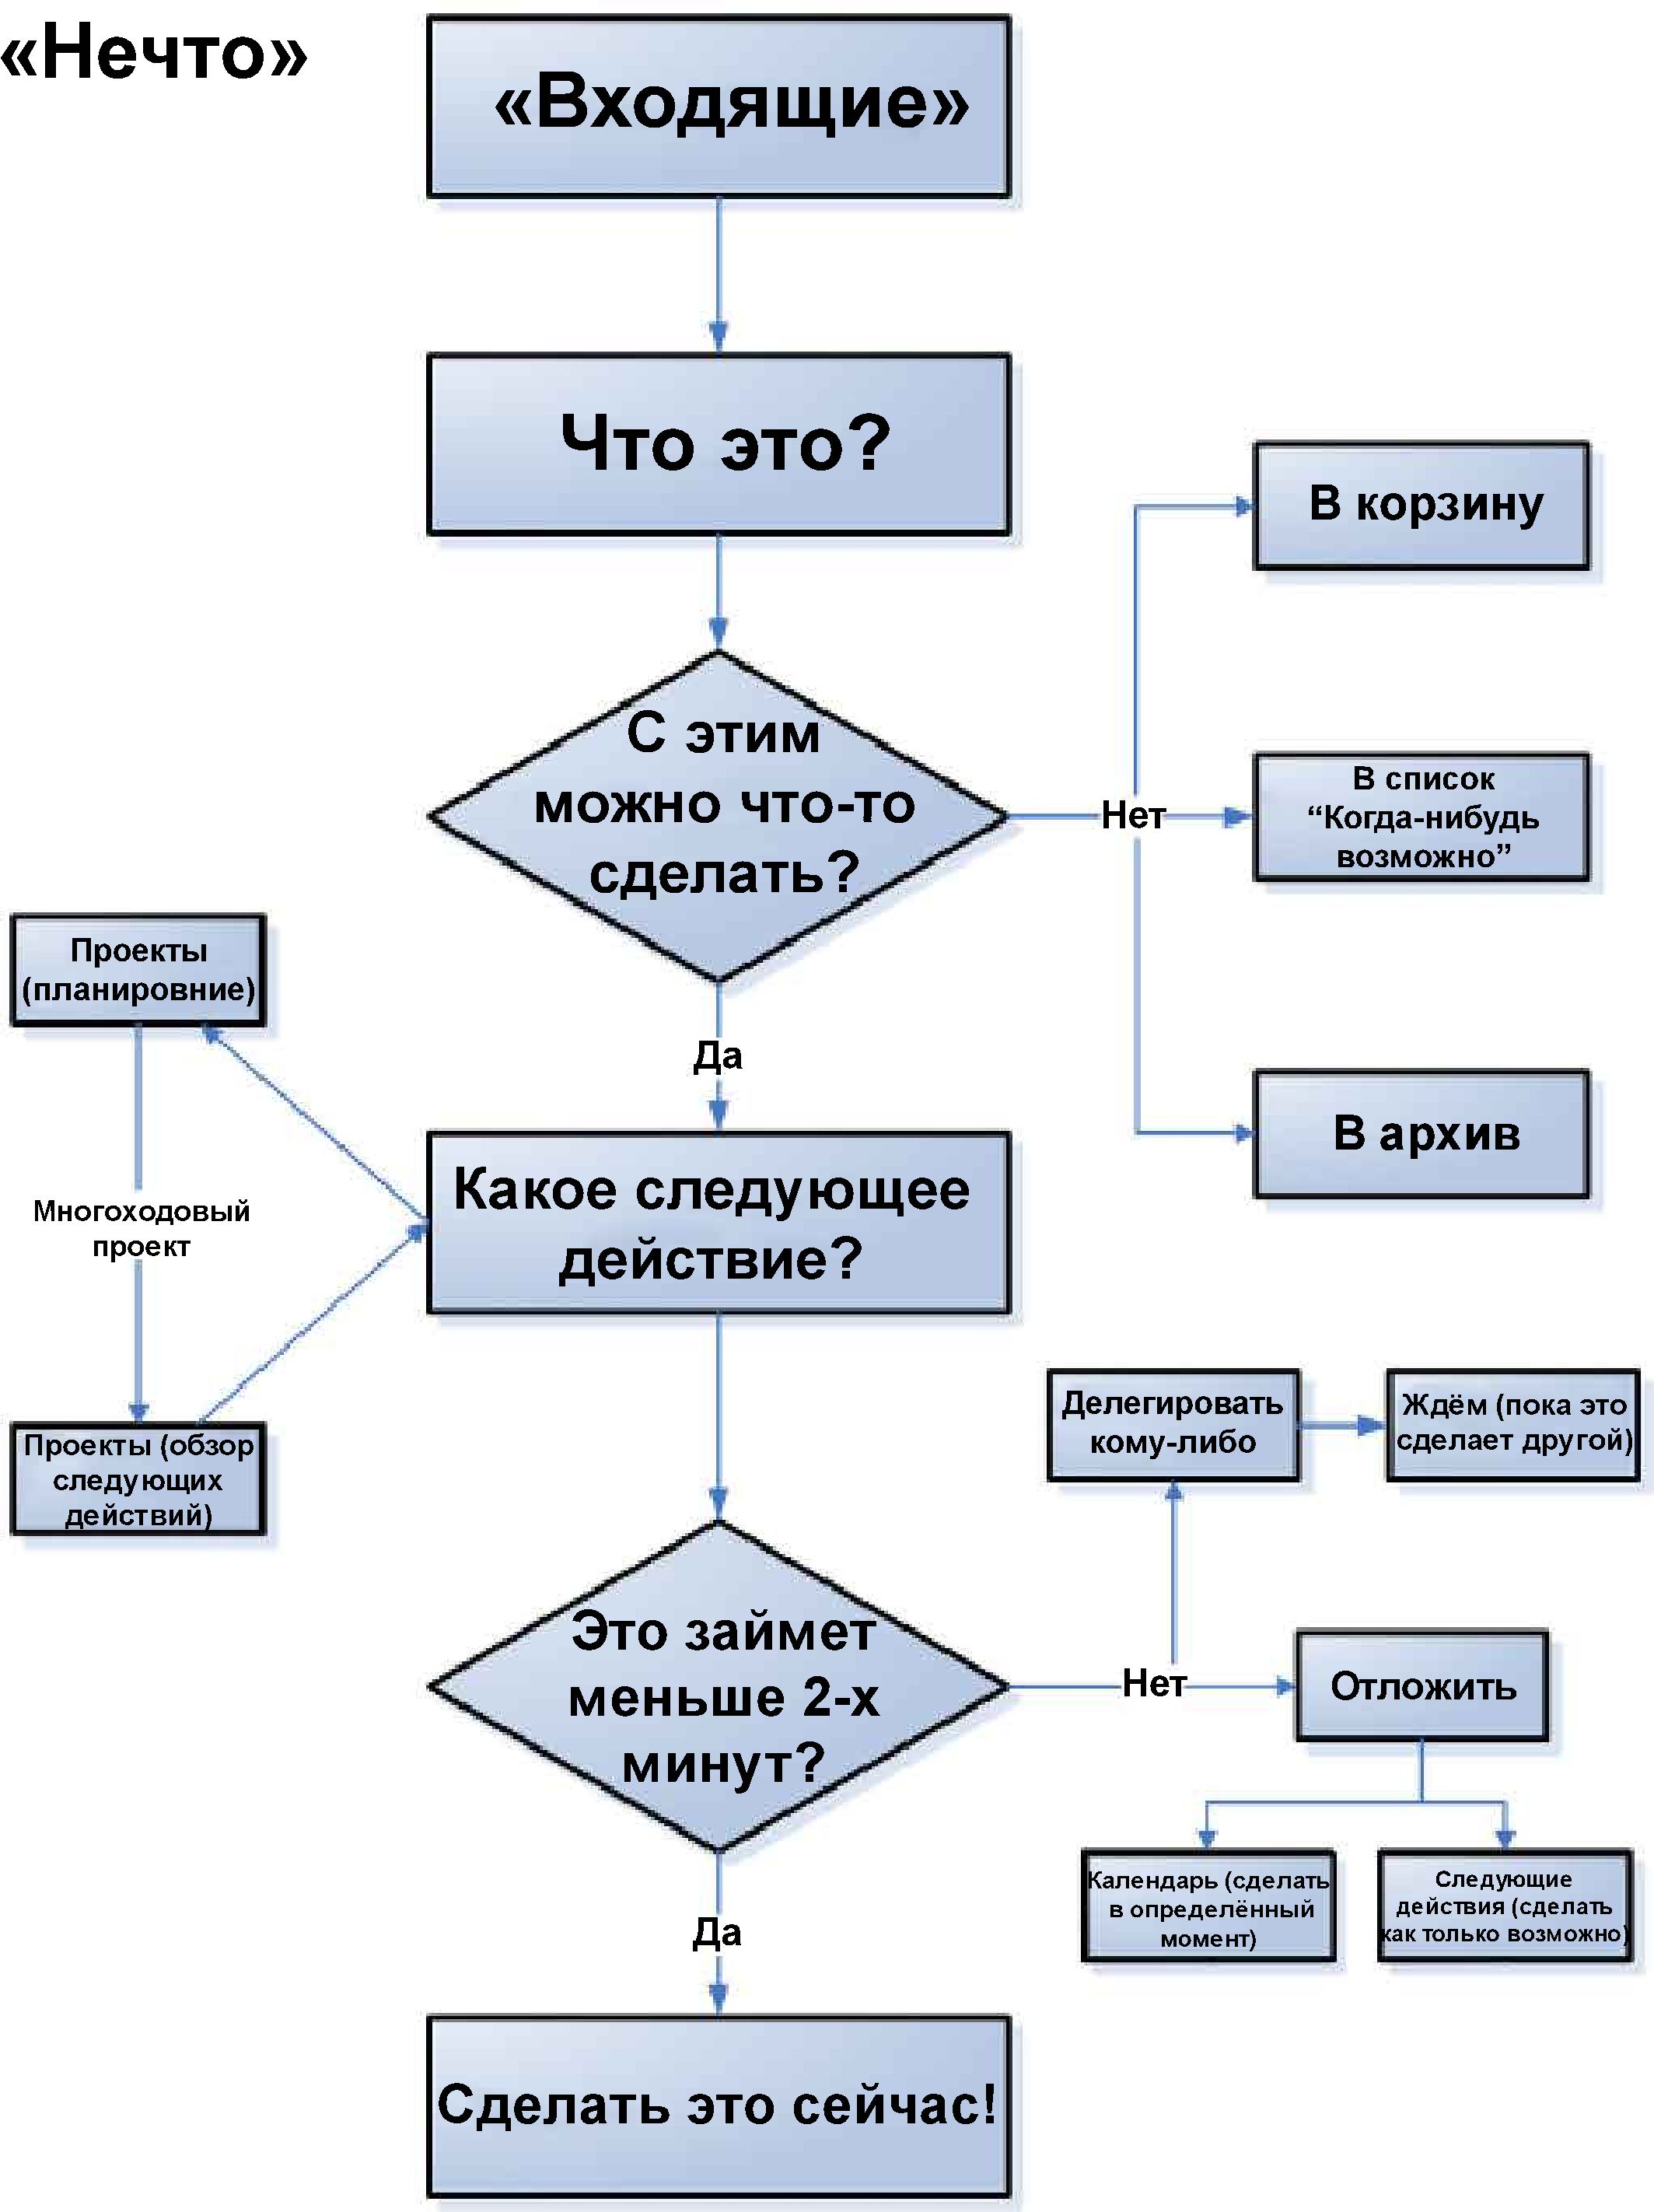
\includegraphics[width=0.5\textwidth]{ProcessingGTD.pdf}}
\end{frame}

\lecturenotes

Обработка корзины идёт строго по следующему алгоритму.
\begin{enumerate}
\item Начинаем с верхнего элемента корзины
\item Делаем один элемент за раз (при этом никогда ничего не возвращаем обратно)
  \begin{itemize}
  \item Если элемент требует действия:
    \begin{itemize}
    \item Делаем это (если на это требуется меньше двух-пяти минут), ИЛИ
    \item Делегируем это кому-нибудь, ИЛИ
    \item Откладываем это
    \end{itemize}
  \item Если элемент не требует действия:
    \begin{itemize}
    \item Оставляем это в справочной информации, ИЛИ
    \item Выбрасываем это, ИЛИ
    \item В список «когда-нибудь может быть»
    \end{itemize}
  \end{itemize}
\end{enumerate}
Если на действие требуется менее чем две-пять минут, это должно быть немедленно сделано. Двухминутное правило обусловлено тем примерным временем, которое нужно, чтобы формально отложить действие~\cite{GTDWikipedia}.

\begin{frame} \frametitle{Процесс обработки}
Важно учесть несколько нюансов:
  \begin{itemize}
  \item Отложить несрочные задачи, например, изучение непрофильных материалов, никак не~связанных с~текущей работой
  \item По~возможности делегировать задачи, например, коллегам или~фрилансерам
  \item Научиться говорить людям «нет», если не~хочется портить отношения с~человеком можно отправить несколько мануалов просящему помощи
  \end{itemize}
\end{frame}

\lecturenotes

С точки зрения работы над ключевым для вас проектом важно учесть несколько нюансов.

\begin{itemize}
\item Отложить несрочные задачи, например, изучение непрофильных материалов, никак не~связанных с~текущей работой
\item По возможности делегировать задачи, например, коллегам или фрилансерам. Если вы быстро и эффективно пишете код, но не очень хорошо справляетесь с задачами создания сайта, рекламы или дизайна, обратитесь к профессионалам. Даже, если это ваш собственный проект, вложение в чужую качественную работу быстро окупится
\item Научиться говорить «нет». Это, пожалуй, один из самых сложных навыков: всегда найдутся десятки знакомых, у которых слетела Windows, закралась ошибка в код, требует прошивки Android и молит о джейлбрейке iPhone. Эти небольшие задачи отнимают массу времени. Если не хотите портить отношения, найдите несколько доступных мануалов в Сети и отправляйте страждущим ссылки~\cite{GTDHabr}
\end{itemize}

\begin{frame} \frametitle{Организация списка}
  \begin{itemize}
  \item Разделить время на~недели, в~конце недели пересматривать список и~создавать новый
  \item Все~задачи разделяются по~срокам выполнения и~по~приоритету
  \item Для~составления наглядной структры проекта можно воспользоваться ассоциативными картами (mindmap), которые отразят все~этапы работы в~виде наглядной структуры-карты
  \item Не~стоит делить задачи на~простые и~сложные, нужно выполнять всё~по~порядку, тогда и~время будет~распределено рационально
  \end{itemize}
\end{frame}

\lecturenotes

После того, как пройдены два первых и самых сложных этапа, необходимо организовать работу с задачами. Тут можно воспользоваться простым правилом: разделить время на недели, в конце недели пересматривать список и создавать новый. Все задачи стоит разделять по срокам выполнения и приоритету. Для ведения задач можно использовать любое из понравившихся приложений: это и мобильные OneNote и Evernote, и Asana, и Redmine, и Google Календарь, и проч…

На этом этапе главное — уделить много внимания работе с текущим или несколькими проектами. Для этого можно воспользоваться ассоциативными картами (mindmap), которые отразят все этапы работы в виде наглядной структуры-карты, в соответствии с которой вы будете продвигаться по проекту. Для создания mindmap существует множество платных и бесплатных приложений с интересными фичами.

Не стоит делить задачи на простые и сложные, нужно выполнять всё по порядку, тогда и время будет распределено рационально~\cite{GTDHabr}. 

\begin{frame} \frametitle{Обзор и Действие}
Обзор сделанного
  \begin{itemize}
  \item На~этом этапе необходимо отметить сделанное, проанализировать причины провалов, создать план на~следующий этап (например, неделю)
  \end{itemize}
Действие
  \begin{itemize}
  \item Выполнять задачи следует исходя из~наличных ресурсов: сил, времени, места выполнения, а~также установленного приоритета
  \item Если для~быстрого решения задачи не хватает какого-то ресурса, который появится позже, нужно~постараться перенести задачу на~момент появления средства её~лучшего исполнения
  \end{itemize}
\end{frame}

\lecturenotes

Ревизия сделанного. На этом этапе необходимо отметить сделанное, проанализировать причины провалов, создать план на следующий этап (например, неделю).

Собственно действие. Выполнять задачи следует исходя из наличных ресурсов: сил, времени, места выполнения, а также установленного приоритета. Если для быстрого решения задачи вам не хватает какого-то ресурса, который появится позже, постарайтесь перенести задачу на момент появления средства её лучшего исполнения. Например, если вы занимаетесь доработкой десктопного приложения и для внесения части изменений требуется обновлённая и ещё не купленная вашей компанией, но запланированная к покупке в ближайшее время SDK, вносите те изменения, которые можно сделать в текущей версии, а задачу по остальным изменениям внесите в папку или файл с задачами на будущее. Безусловно, поиск путей решения задачи имеющимися средствами раскрывает вас как профессионала, но требует больших и не всегда оправданных затрат вашего времени и сил~\cite{GTDHabr}.

\begin{frame} \frametitle{Как использовать принципы GTD}
  \begin{itemize}
  \item Планировать проект изначально, а~не по~ходу работы, дробить его на~решаемые подзадачи
  \item Выделять отдельные этапы работы над~проектом и~проставлять метки важности и~срочности выполнения работы
  \item Доводить каждую задачу до~конца, не~оставляя её на~потом
  \item Периодически пересматривать списки задач с~целью ревизии выполненного и~изменения планов
  \item В~один момент времени сосредотачиваться на~одной задаче
  \item Выделять время на~каждый этап и~уделять ему~максимальное внимание
  \end{itemize}
\end{frame}

\lecturenotes

Вот несколько советов, как использовать принципы GTD, если вы разработчик в команде или работаете самостоятельно.

  \begin{itemize}
  \item Планируйте свой проект изначально, а не по ходу работы, дробите его на решаемые подзадачи
  \item Выделяйте отдельные этапы работы над проектом и проставляйте метки важности и срочности выполнения работы
  \item Доводите каждую задачу до конца, не оставляя её на потом. Даже, если вы знаете только длинный путь решения задачи, решите её. В ходе дальнейшего рефакторинга можно будет избавиться от неоптимального решения
  \item Периодически пересматривайте списки задач с целью ревизии выполненного и изменения планов
  \item В один момент времени сосредоточьтесь на одной задаче — так вы сэкономите время и силы
  \item Выделяйте время на каждый этап и уделяйте ему максимальное внимание: на сбор требований, на разработку, на unit-тестирование и прочее
  \end{itemize}

GTD нельзя внедрить одним днём — сперва появляются какие-то отдельные элементы, затем формируются правила, наконец, появляется привычка и ощутимый результат. Главное — не останавливаться. Кстати, неплохо, если вы сможете перенести часть своих навыков в GTD на команду, с которой работаете — это может значительно оптимизировать работу внутри компании~\cite{GTDHabr}.

\section{Управление взаимодействием с другими сотрудниками}

\begin{frame} \frametitle{Коммуникация}
  \begin{itemize}
  \item Разработчику каждый день нужно взаимодействовать с~другими сотрудниками
  \item Существует большое количество способов коммуникации, и~все они имеют разную эффективность
  \end{itemize}
\end{frame}

\begin{frame} \frametitle{Эффективность различных видов коммуникации}
\centerline{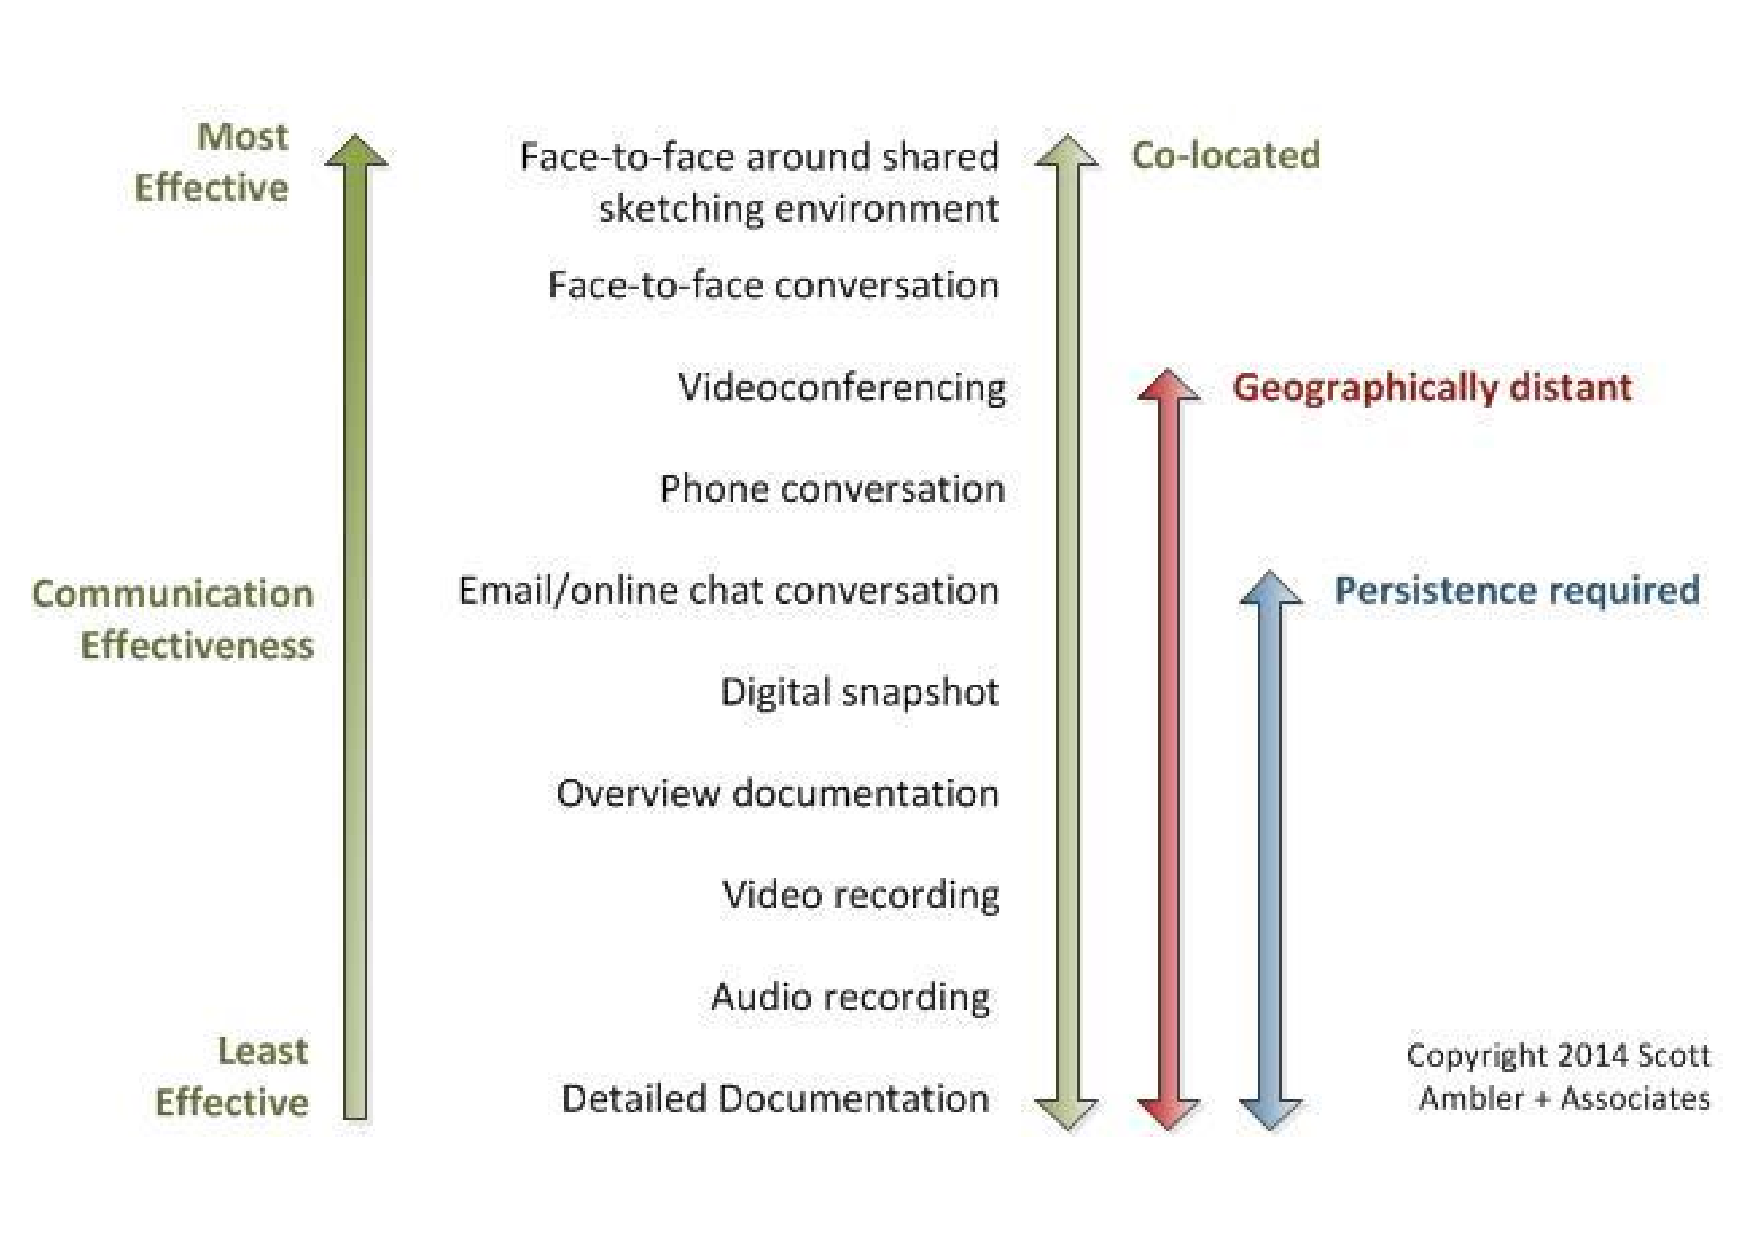
\includegraphics[width=0.8\textwidth]{CommunicationEffectiveness.pdf}}
\end{frame}

\lecturenotes

Наиболее эффективная коммуникация от человека к человеку, лицом к лицу, особенно когда она улучшается с помощью совместного модельного средства, такого как доска (POW), флип-чарт, бумага. Когда вы удаляетесь от этой ситуации, возможно, удалив общий носитель или больше не сталкиваясь с лицом, вы испытываете снижение эффективности общения. По мере того как богатство вашего канала связи охлаждается, вы теряете физическую близость и сознательные и подсознательные подсказки, которые обеспечивает такая близость. Вы также теряете выгоду от нескольких модальностей, способности общаться через методы, отличные от слов, таких как жесты и выражения лица. Также теряется способность изменять вокальную флексию и время, люди не только общаются через слова, которые они говорят, но и как говорят эти слова. Кокберн указывает, что говорящий может подчеркнуть то, что они говорят, таким образом изменяя способ общения, ускоряя, замедляя, приостанавливая или меняя тона. Наконец, способность отвечать на вопросы в реальном времени, точка, которая отличает кривую параметров моделирования от кривой параметров документации, важна, потому что вопросы дают представление о том, насколько хорошо информация понимается слушателем~\cite{AgileComm}.

\begin{frame} \frametitle{Принципы коммуникации}
  \begin{itemize}
  \item Нужно стремиться к~наиболее эффективному способу коммуникации, возможному в~текущей ситуации
  \item Эффективность различных стратегий коммуникации может меняться, нужно пробовать новые, а~не~зацикливаться на~каком-то одном
  \end{itemize}
\end{frame}

\lecturenotes

Стремитесь следовать наиболее эффективному методу коммуникации, применимому к вашей ситуации. Если вы работаете вместе с кем-то в одной комнате, скорее всего, вам лучше обсудить что-то с ними лицом к лицу на доске, чем написать им документ, который вы в конечном итоге передадите им. Если вы работаете с кем-то в другом месте, вам нужно будет установить с ними обычные видеоконференции, иметь общий репозиторий информации и регулярно отправлять по электронной почте.
Будьте готовы изменить свой подход во всем проекте. Динамика команды будет меняться по всему проекту, поэтому стратегия коммуникации, которая хорошо зарекомендовала себя вчера, может плохо работать сегодня. Ежедневная конференц-связь, которую вы представили три месяца назад для решения проблем связи между членами распределенной команды, теперь больше не понадобится, когда люди создали взаимопонимание и теперь используют общее программное обеспечение для чата и при необходимости делают импровизированные звонки. Подразумевается, что вы должны регулярно сомневаться в способах общения, хорошим вариантом является сделать это в конце каждой итерации во время ретроспективного улучшения процесса~\cite{AgileComm}.

\begin{frame} \frametitle{Факторы эффективной коммуникации}
  \begin{itemize}
  \item Физическая близость --- чем~ближе люди друг к~другу физически, тем~больше возможностей для~общения
  \item Временная близость --- если~сотрудники работают в~примерно одинаковых часовых поясах, то~им гораздо проще взаимодействовать
  \item Дружелюбие --- это желание понять мысли другого человека, говорить добродушно. Чем~больше дружелюбия, тем~качественее передаётся информация
  \end{itemize}
\end{frame}

\lecturenotes

Существует несколько факторов, влияющих на общение, в том числе:

Физическая близость. Чем ближе люди к друг другу, тем больше возможностей для общения. На одном конце спектра два человека могут работать параллельно с парным программированием на одной рабочей станции, а на другом конце спектра два человека могут находиться в разных зданиях.

Временная близость. Независимо от того, воздействуют ли одновременно два человека на общение. Вы можете быть отделены от некоторых ваших сотрудников несколькими часовыми поясами, для североамериканских фирм довольно часто аутсорсинг работы в области развития для азиатских или европейских компаний или даже просто по разным личным графикам. Однажды я переехал из Торонто в Сан-Франциско, чтобы работать над контрактом на разработку, проводя четыре дня в неделю в Сан-Франциско. Я быстро понял, что не могу постоянно менять свои внутренние часы, чтобы соответствовать часовому поясу, в котором я был, между городами разница в три часа, поэтому решил остаться в Торонто. Будучи утренним человеком, я просыпался в 3 часа ночи в Сан-Франциско, однако многие из моих сотрудников были ночными людьми и обычно работали до 3 или 4 утра. Мы обнаружили, что это довольно эффективно: я работал бы днем ​​и оставался в офисе, пока они не начали прибывать, разговаривая лицом к лицу с ними по мере необходимости. Затем я отправился в свой отель, спал и начал общаться с электронной почтой сразу после пробуждения, позволяя мне узнать, над чем они работали в течение ночи, а затем помогать по электронной почте там, где это необходимо. Это было не идеально, но мы заработали.

Дружелюбие. Кокберн считает, что важным фактором успеха является дружелюбие, желание кого-то услышать мысли другого человека с доброй волей и говорить без злого умысла. Чем больше дружелюбие будет передаваться большее количество и качество информации, тем меньше будет скрыто. Добровольство тесно связано с доверием, которое люди имеют друг к другу, и чувством сообщества, которым они разделяют. Кокберн сообщает, что иногда дружба может быть слишком высокой, люди могут так беспокоиться о том, чтобы оскорбить своих коллег, что они боятся не согласиться с ними или боятся взять инициативу из страха быть воспринятыми как искатели славы~\cite{AgileComm}.

\begin{frame} \frametitle{Коммуникация с другими отделами}
  \begin{itemize}
  \item Прямое общение с~сотрудником другого отдела
  \item Общение с~менеджером, руководящим другим отделом
  \item Общение на~совместных совещаниях, планёрках и т.д.
  \end{itemize}
\end{frame}

\section{Инструменты организации деятельности отдельного разработчика}

\begin{frame} \frametitle{Tomato Timer}
  \begin{itemize}
  \item Представляет удобный интерфейс для~использования техники Pomidoro
  \item Позволяет скачать дополнительные материалы для~более удобного отслеживания периодов
  \item Можно использовать как на~компьютере так~и на~мобильном устройстве
  \end{itemize}
\end{frame}

\begin{frame} \frametitle{tomatotimer.ru}
\centerline{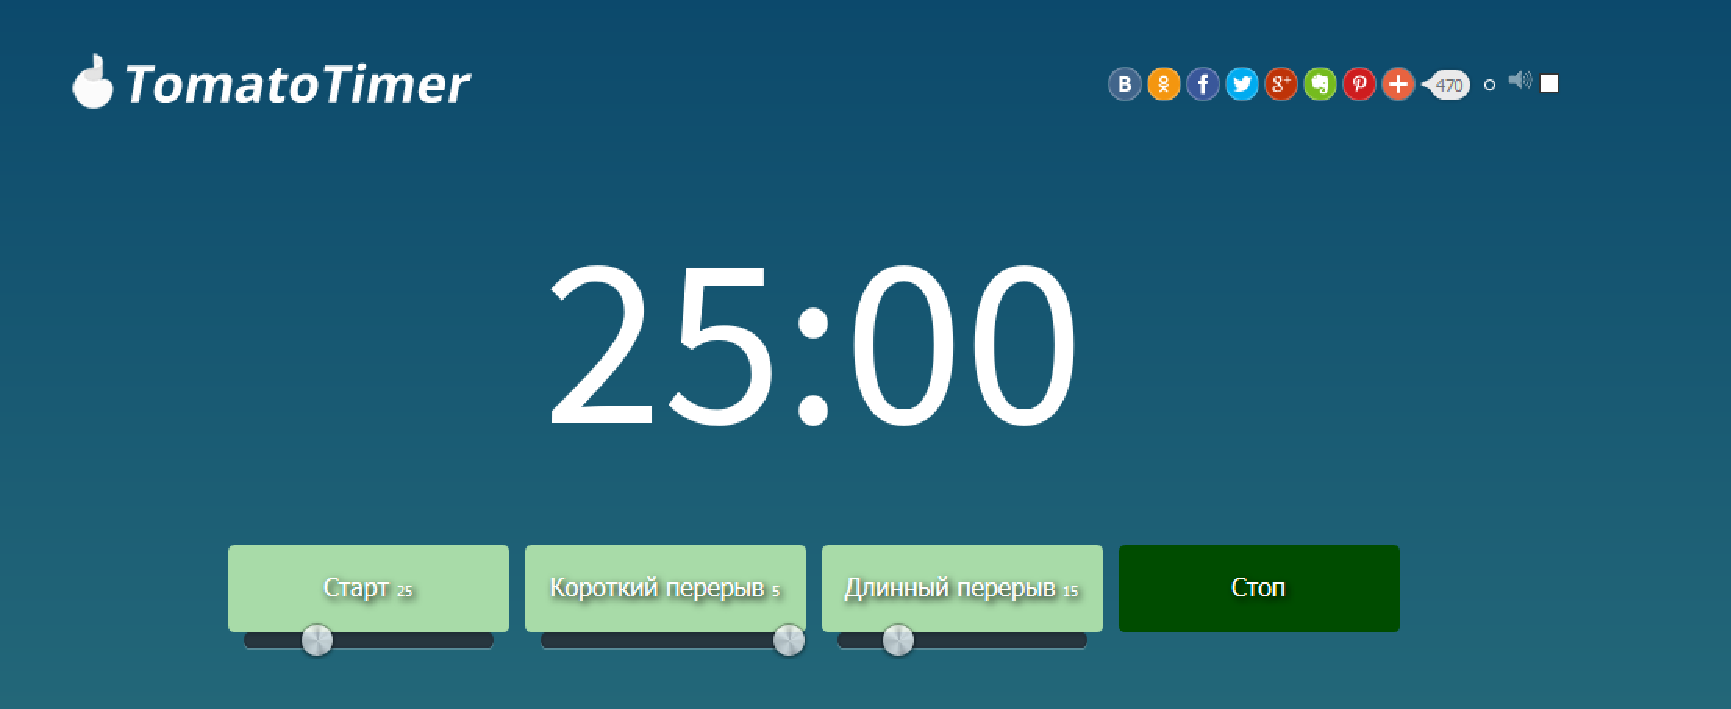
\includegraphics[width=1\textwidth]{tomatotimer.pdf}}
\end{frame}

\begin{frame} \frametitle{Trello}
  \begin{enumerate}
  \item Все новоприходящие дела записываются в~папку «Входящие»
  \item К~каждому делу можно добавляется информация: время, место и~т.д.
  \item Они рассортировываются по~папкам
  \end{enumerate}
\end{frame}

\begin{frame} \frametitle{trello.com}
\centerline{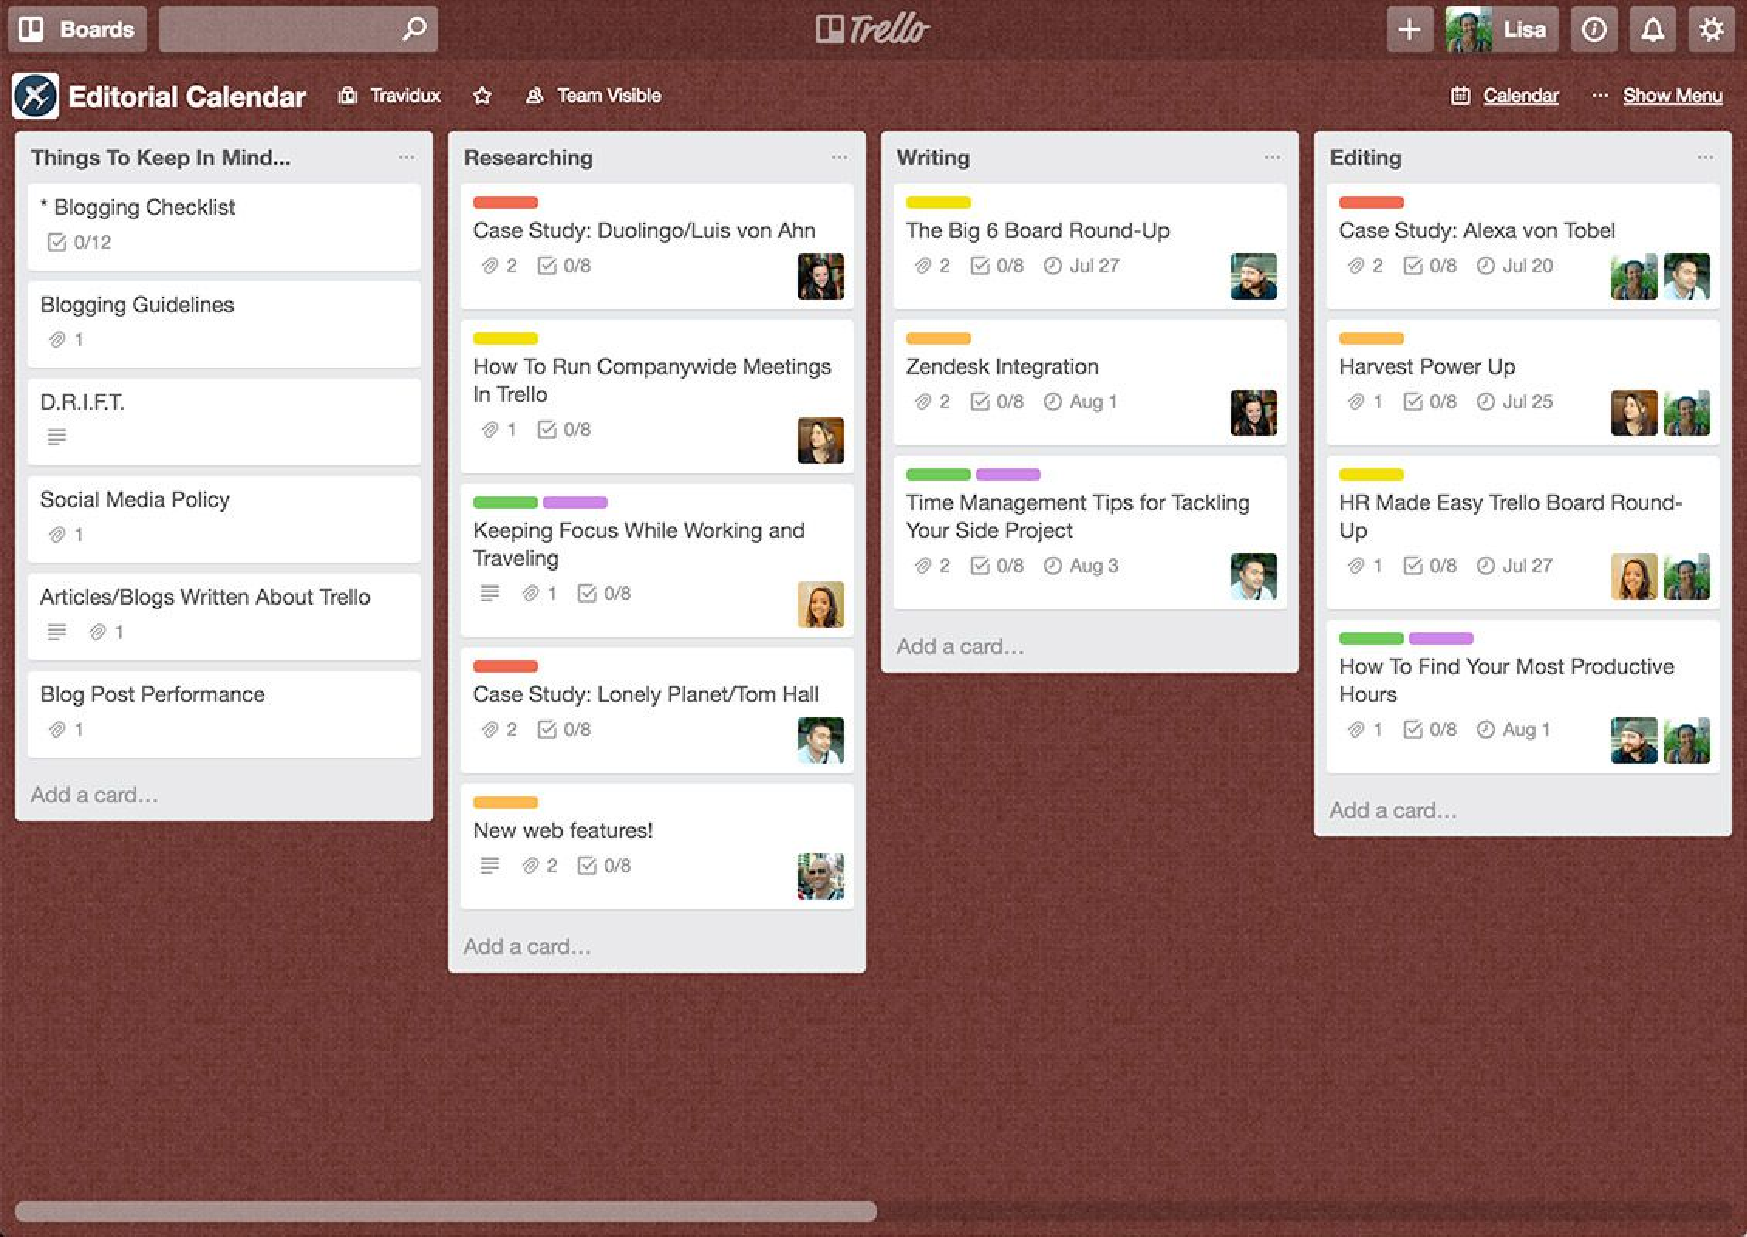
\includegraphics[width=0.9\textwidth]{trello.pdf}}
\end{frame}

\begin{thebibliography}{99}
\bibitem{TMHabr} \href{https://habrahabr.ru/post/259293/}{Тайм-менеджмент для разработчика / Хабрахабр}
\bibitem{TasksMedium} \href{https://medium.com/@skidanolegs/анализ-задачи-и-разбиение-задач-на-подзадачи-21b7865f387f}{Анализ задачи и разбиение задач на подзадачи – Oleg Skidan – Medium}
\bibitem{TasksHabr} \href{https://habrahabr.ru/post/111873/}{Разбиение на подзадачи: почему работает, и почему нет / Хабрахабр}
\bibitem{TMCodeProject} \href{https://www.codeproject.com/Articles/11502/Time-Management-Tips-for-Developers}{Time Management Tips for Developers - CodeProject}
\bibitem{TMSeimer} \href{https://lostechies.com/andrewsiemer/2016/01/04/developer-personal-time-management/]}{Developer personal time management | Andrew Seimer}
\bibitem{Pomidoro} \href{https://happydiva.ru/time-management/273-upravlenie-vremenem-metod-pomidora-pomodoro}{Управление временем: метод помидора (pomodoro)}
\bibitem{GTDWikipedia} \href{https://ru.wikipedia.org/wiki/Getting_Things_Done}{Getting Things Done — Википедия}
\bibitem{GTDHabr} \href{https://habrahabr.ru/company/geekbrains/blog/270865/}{Прочь из моей головы. GTD в разработке / Блог компании GeekBrains / Хабрахабр}
\bibitem{AgileComm} \href{http://agilemodeling.com/essays/communication.htm}{Communication on Agile Software Teams}
\end{thebibliography}

\end{document}

%%% Local Variables: 
%%% mode: TeX-pdf
%%% TeX-master: t
%%% End: 
